\chapter{Evaluation}
\renewcommand{\baselinestretch}{\mystretch}
\label{chap:Eval}
%\setlength{\parindent}{0pt}

\section{Locale issue}

Initially, the Vixen project was unable to be built on the Windows system. The problem was caused by different system locale setting from English to Chinese, affecting the file encoding the compiler assumes. Special characters such as \"a were misunderstood as other string literals, failed the compilation.

There are 2 possible solutions to the problem. The system locale can be changed, or specify the actual file encoding to the compiler. In order to have a permanent solution, the \texttt{CodePage} setting was specified in the project file \cite{codepage}, although the setting itself was undocumented for project files.

\section{Original performance}

The original Vixen application already has an built-in instrumentation display interface that can show runtime performance figures such as controller update speeds. However, it lacks some elemental functionalities for performance analysis. Data logging, playback timestamps and CPU usage logging were added for performance analysis.

The Vixen application uses a separate thread for each task. It has the main GUI thread for editor, a preview rendering thread and multiple dedicated threads for active controllers. This multi-threading structure can take advantage of modern multi-core multi-thread processors. However, performance on a single core machine can be poor due to context switching. Mutex locks are also required to resolve potential data access conflict, further increases the overhead.

\fref{fig:original} shows the performance of the original Vixen execution engine. The CPU usage frequently reaches above $90 \%$, while the refresh rate being very unstable around the configured 20 fps. Especially at the first 60 seconds, the refresh rate drops to 5 fps while trying to keep up with element updates. At the same time, the CPU usage was about $50 \%$. On a dual-core machine, this implies one of the cores was running at full load while the other one was mostly idle. \wn{2}

\begin{figure}[t]
  \centering
  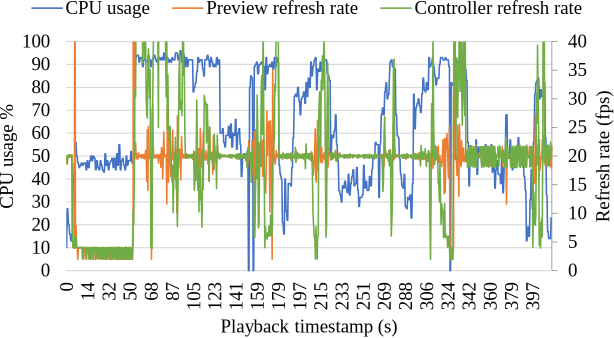
\includegraphics[width=0.8\columnwidth]{original}
  \caption{Performance of original Vixen execution engine}
  \label{fig:original}
\end{figure}

Further analysis using Microsoft Visual Studio's sampling profiler shows, around $24.7 \%$ of total CPU time was wasted between translation layers for generating controller commands (\texttt{GenerateCommand}), while the actual command assignment (\texttt{\_8BitEvaluator}) takes less than $0.5 \%$ of CPU time, as shown by \fref{fig:vixen_perf_original} hot path analysis. Another $23.0 \%$ CPU time was used for filter and element updates, $26.0 \%$ for preview rendering and $16.9 \%$ for the sequence editor, as shown by \fref{fig:vixen_perf_original_overview}. The CPU time used for controller updates is almost negligible.

\begin{figure}[t]
  \centering
  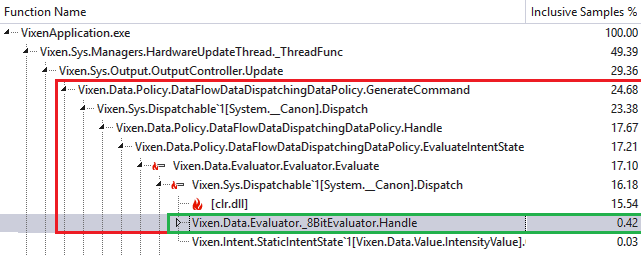
\includegraphics[width=0.85\columnwidth]{Figs/vixen_perf_original.png}
  \caption{Hot path analysis of Vixen update threads}
  \label{fig:vixen_perf_original}
\end{figure}

\begin{figure}[t]
  \centering
  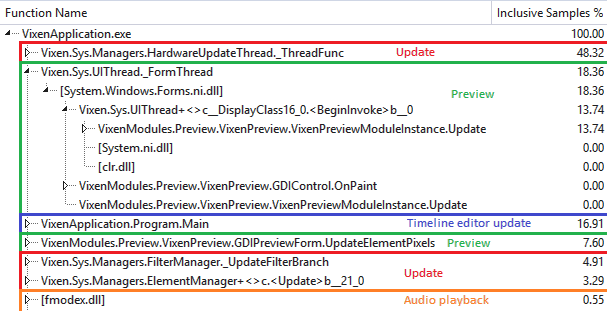
\includegraphics[width=0.85\columnwidth]{Figs/vixen_perf_original_overview.png}
  \caption{Hot path analysis of original Vixen application}
  \label{fig:vixen_perf_original_overview}
\end{figure}

The translation layers are used for determining the actual controller command format. There are several different command formats possible for varies controllers. For example, 8-bit, 16-bit or RGB channels. Therefore, the application need to resolve the actual types of commands for specific assignment handlers from a common command base type, which apparently very inefficient in C\#. This process is called \texttt{dispatch} in the source code, it must be minimised in order to improve performance. \wn{3}

The implementation of preview display was also very inefficient, uses only software instance management and sequential rendering. It can be improved by the utilisation of GPU through DirectX or OpenGL.

Multiple real-world lighting sequences and testing sequences were tested. They all show similar performance characteristics with unstable playback frame rate for moderately complicated lighting effects.

\section{Port to Linux}

It takes some necessary modifications for Vixen to run on Linux using mono runtime. The MonoDevelop IDE \cite{monodevelop} helps by directly supporting Microsoft Visual Studio projects. However, C/C++ projects were not supported, and pre-built dynamic runtime libraries developed using C/C++ for Microsoft Windows were also not support by mono. All code references to WPF and FMOD audio must be removed for the project to build and run.

The result Vixen application for Linux has a distorted main GUI with unreasonably long vertical window size. The sequence editor, display setup and preview would either not load or crash the entire application. Fortunately, all controller modules can be loaded and the core execution engine and controller update threads were working properly. \fref{fig:vixen_linux_main} shows some loaded controller modules and partially working GUI.

\begin{figure}[t]
  \centering
  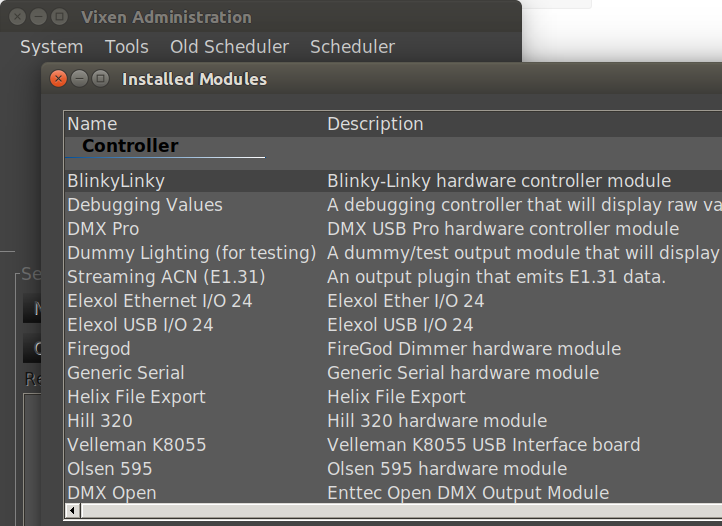
\includegraphics[width=0.8\columnwidth]{Figs/vixen_linux_controllers.png}
  \caption{Controller modules loaded on Linux port of Vixen application}
  \label{fig:vixen_linux_main}
\end{figure}

The intended optimised Vixen application would be command-line user interface (CUI) only with minimal essential functionality. Therefore, the broken GUI should not be an issue.

\section{Extract rendered sequence}

Instead of trying to improve the original execution engine, the performance problem may be eliminated by playing pre-rendered controller layer data frames directly to individual hardware controllers. Channel data type information can be stored separately without the need to resolve through translation layers during runtime. Element updates, Filter updates, preview and sequence editor are all necessary for playback.

Two steps are needed for this approach. Firstly, pre-render the sequence with precise frame interval, then playback the rendered data to the controllers as a separate process and perhaps on an entirely different platform.

To pre-render the sequence, two different methods are possible. A dummy controller can be used for runtime data dumping, or use a separate export engine with manual frame control independent of wall-clock time.

\section{Custom controller}
\label{sec:tcplinky}

A custom controller module (\texttt{TCPLinky}) was developed based on one of its existing controller (\texttt{BlinkyLinky}). This controller uses TCP connection to transfer display channel data, supports up to 65535 channels. A corresponding cross-platform server application that simulates a multi-channel display was also developed using C++ with Qt \cite{qt} and OpenGL \cite{shreiner2009opengl} rendering. This server application allows real-time debugging of display output without the need of a complex physical lighting system setup. Data dumping, performance and statistical analysis can also be easily achieved. \wn{4}

\fref{fig:tcplinky_server} shows a screenshot of the server application. With the help of GPU rendering through OpenGL, it consumes less than $3 \%$ of CPU time under 50 fps refresh rate, which is negligible. It can also be compiled and executed on other computers, simulates real world network connected controller scenarios.

\begin{figure}[t]
  \centering
  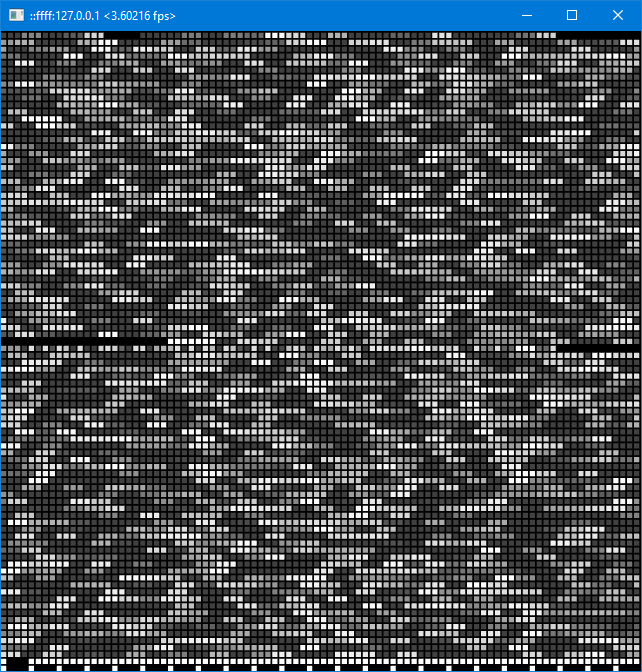
\includegraphics[width=0.6\columnwidth]{Figs/tcplinky_server.png}
  \caption{Screenshot of \texttt{TCPLinky} controller server application}
  \label{fig:tcplinky_server}
\end{figure}

\section{Export sequence}

Although the custom controller module is capable of dumping outputs, it can not give the indication of sequence start, end and information about other controllers. More notably, it can have unstable frame rates influenced by CPU usage. A high performance computer is needed for near prefect pre-rendering by controller dump. Therefore, the existing sequence export function from sequence editor was used instead.

The export function was originally used to convert the lighting sequence to formats recognisable by other controller specific applications. It renders the sequence using a manual timing source stepped after each frame, gives accurate constant data dump intervals. It can also write all controller channel mapping information to a separate XML file. An example XML file is shown by \lref{lst:network_xml}.

\begin{lstlisting}[float,floatplacement=t,language=XML,label=lst:network_xml,captionpos=b,caption={Example controller mapping XML file}]
<?xml version="1.0" encoding="utf-8"?>
<Vixen3_Export>
  <Resolution>20</Resolution>
  <OutFile>luf2013_20ms.raw</OutFile>
  <Duration>00:04:45.8050000</Duration>
  <Network>
    <Controller>
      <Index>0</Index>
      <Name>E6804 arches L</Name>
      <StartChan>1</StartChan>
      <Channels>2048</Channels>
    </Controller>
    <Controller>
      <Index>1</Index>
      <Name>Lynx DMX</Name>
      <StartChan>2049</StartChan>
      <Channels>156</Channels>
    </Controller>
  </Network>
  <Media>
    <FilePath>example_audio.mp3</FilePath>
  </Media>
</Vixen3_Export>
\end{lstlisting}

To support the purposed optimised playback engine, audio media file path was added to the XML. The export dialog window was modified to allow custom frame resolution through text input, instead of a few pre-defined fixed values on the drop down list, as shown by \fref{fig:vixen_export}. Additional data format entries such as the ``Raw File"" for the playback engine was also added to the export wizard. \wn{5}

\begin{figure}[t]
  \centering
  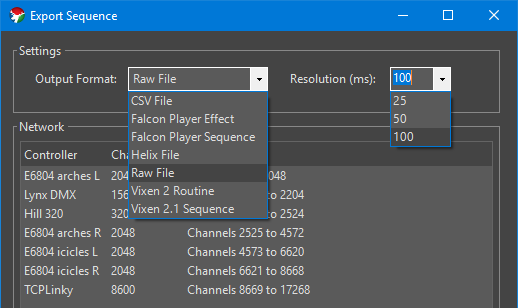
\includegraphics[width=0.75\columnwidth]{Figs/vixen_export.png}
  \caption{Modified Vixen export dialog window}
  \label{fig:vixen_export}
\end{figure}

\section{Source code management}

All source code related to Vixen and other programs developed in this project were managed using git version control tool \cite{git}, hosted on GitHub \cite{github} \cite{github_vixen_yz} \cite{github_project}.

Using a version control system enables history changes tracking for source code. Together with a web-based hosting service like GitHub, changes to the source code can be easily backup and synchronised on multiple devices and the cloud. The source code for official Vixen application was also hosted on GitHub \cite{github_vixen}. With GitHub's signature fork and pull request functionality, straightforward cooperation between different organisations and people can be achieved. The modifications made in this project can be therefore easily incorporated into the official Vixen application source code repository for public use.
